%%%%%%%%%%%%%%%%%%%%%%%%%%%%%%%%%%%%%%%%%
% University Assignment Title Page LaTeX Template Version 1.0 (27/12/12)
%
% This template has been downloaded from: http://www.LaTeXTemplates.com
%
% Original author: WikiBooks (http://en.wikibooks.org/wiki/LaTeX/Title_Creation)
%
% License: CC BY-NC-SA 3.0 (http://creativecommons.org/licenses/by-nc-sa/3.0/)
% 
% Instructions for using this template: This title page is capable of being compiled as is. This is not useful for
% including it in another document. To do this, you have two options: 
%
% 1) Copy/paste everything between \begin{document} and \end{document} starting at \begin{titlepage} and paste this into
% another LaTeX file where you want your title page.  OR 2) Remove everything outside the \begin{titlepage} and
% \end{titlepage} and move this file to the same directory as the LaTeX file you wish to add it to.  Then add
% \input{./title_page_1.tex} to your LaTeX file where you want your title page.
%
%%%%%%%%%%%%%%%%%%%%%%%%%%%%%%%%%%%%%%%%%
%\title{Title page with logo} ----------------------------------------------------------------------------------------
%PACKAGES AND OTHER DOCUMENT CONFIGURATIONS
%----------------------------------------------------------------------------------------

\documentclass[12pt]{article} \usepackage[english]{babel} \usepackage[utf8x]{inputenc} \usepackage{amsmath}
\usepackage{graphicx} \usepackage[colorinlistoftodos]{todonotes}

\begin{document}

\begin{titlepage}

\newcommand{\HRule}{\rule{\linewidth}{0.5mm}} % Defines a new command for the horizontal lines, change thickness here

\center % Center everything on the page
 
%---------------------------------------------------------------------------------------- HEADING SECTIONS
%----------------------------------------------------------------------------------------

\textsc{\LARGE Nanyang Technological University}\\[1.5cm] % Name of your university/college \textsc{\Large School of
Computer Engineering}\\[0.5cm] % Major heading such as course name \textsc{\large Interim Report}\\[0.5cm] % Minor
heading such as course title

%----------------------------------------------------------------------------------------

%	TITLE SECTION
%----------------------------------------------------------------------------------------

\HRule \\[0.4cm] { \huge \bfseries Title}\\[0.4cm] % Title of your document \HRule \\[1.5cm]
 
%---------------------------------------------------------------------------------------- AUTHOR SECTION
%----------------------------------------------------------------------------------------

\begin{minipage}{0.4\textwidth} \begin{flushleft} \large \emph{Author:}\\ Tuan Phong \textsc{Nguyen} % Your name
\end{flushleft} \end{minipage} ~ \begin{minipage}{0.4\textwidth} \begin{flushright} \large \emph{Supervisor:} \\ Assoc
    Prof Chiew Tong \textsc{Lau} % Supervisor's Name \end{flushright} \end{minipage}\\[2cm]

% If you don't want a supervisor, uncomment the two lines below and remove the section above
%\Large \emph{Author:}\\ John \textsc{Smith}\\[3cm] % Your name

%---------------------------------------------------------------------------------------- DATE SECTION
    %----------------------------------------------------------------------------------------

{\large \today}\\[2cm] % Date, change the \today to a set date if you want to be precise

%---------------------------------------------------------------------------------------- LOGO SECTION
%----------------------------------------------------------------------------------------

%----------------------------------------------------------------------------------------

\vfill % Fill the rest of the page with whitespace

\end{titlepage}

\section{Introduction}
Along with the development of more compact and portable platform for measuring health related data, there are many
products on the market that are capable of reading and sending data to a computer system. These devices are often built
ready for communicating with mobile devices via Bluetooth to exchange data so that those data can be displayed visually.
However, a universal platform to collect and display the data to users has not been implemented yet. On the other hand,
the measured data is not frequently recorded so that it can be used as reference in diagnosing or study.  This project
aims to implement such a platform with consideration on capability of adapting multiple types of devices, data sharing
as well as the scalability.

\section{Architecture design}
\label{sec:Architecture design}
The application contains 3 main components namely the client, the backend server and the database.

\subsection{Client side}
The client is responsible for displaying the data acquired from the physical measuring devices visually as graph or
reading listing. The client application needs to acquire the the data records from the backend server through network
communication and cache it in local database for presenting to the app user. In order to server as a universal interface to
various types of medical record, the interface is capable of displaying different types of graph for different record
type and designed to be extended when there is need for a new representation of data. The client connects 
to the back-end to interact with other users of the application to share and access their data in the database. The
client also provides the user with an interface to search for another users of the application and interact with them.
Users can subscribe to another user to view their data and receive notifications upon certain events are triggered such
as when new data is uploaded or when the reading is beyond safe range. As the database is accessed through a RESTful API
via HTTP request and response, the client application can be implemented in any platform e.g. Android, iOS, native
desktop program or web application. Due to time constraint and man power of this project as well as the extensibility to
other projects, the client is only implemented for android phones.

\subsection{Server side}
The server is a Web server that exposes a RESTful API to the clients and serves the incoming requests. To perform the
business logic, the server interacts with a persistent database to provide the service as application backend. To
elevate scalability of the application, the server side is chosen to be hosted on Google App Engine cloud service. By
using cloud computing from a credible service provider, the application aims to minimize down-time and bottleneck
comparing to self-hosting service on a single computer.  In addition, hosting application on a cloud platform also
enables the application cost to scale better with the number of users and data traffic since the service provider offers
multiple pricing tiers for different amount of traffic.  Moreover, Datastore database provided by Google also supports
caching and reliably distributes data to different locations with minimal latency.  Regarding implementation of ther
server program, since client and server communicate through a RESTful API, the server can also be implemented in any
programming languages. In this project, the web server is implemented in Java with Google Endpoints API.  This helps
promote code reuse by sharing Java object between client and server codebase. In the future, the server can be swapped
out by any web server if there is need for finer control or performance improvement.

\subsection{Database}
Google Cloud Datastore is chosen to be the database backend of the system to reliably store and deliver data. Google
Cloud Datastore is a schema-less NoSQL Datastore providing robust, reliable storage for the web application. In
constrast with SQL-like database, Datastore treats each record in the database as a key-value pair without unnecessary
indexes. Comparing to the traditional relation databases, the Datastore uses a distributed architecture to automatically
managing scaling to very large data sets. Additionally, Datastore is hosted as part of the Google App Engine platform,
hence is fully managed with no planned down time by Google. Due to its different way of representing and managing data,
the Datastore can be easily scaled, allowing the application to maintain high performance as the traffic is increased.

% Commands to include a figure:
\begin{figure} 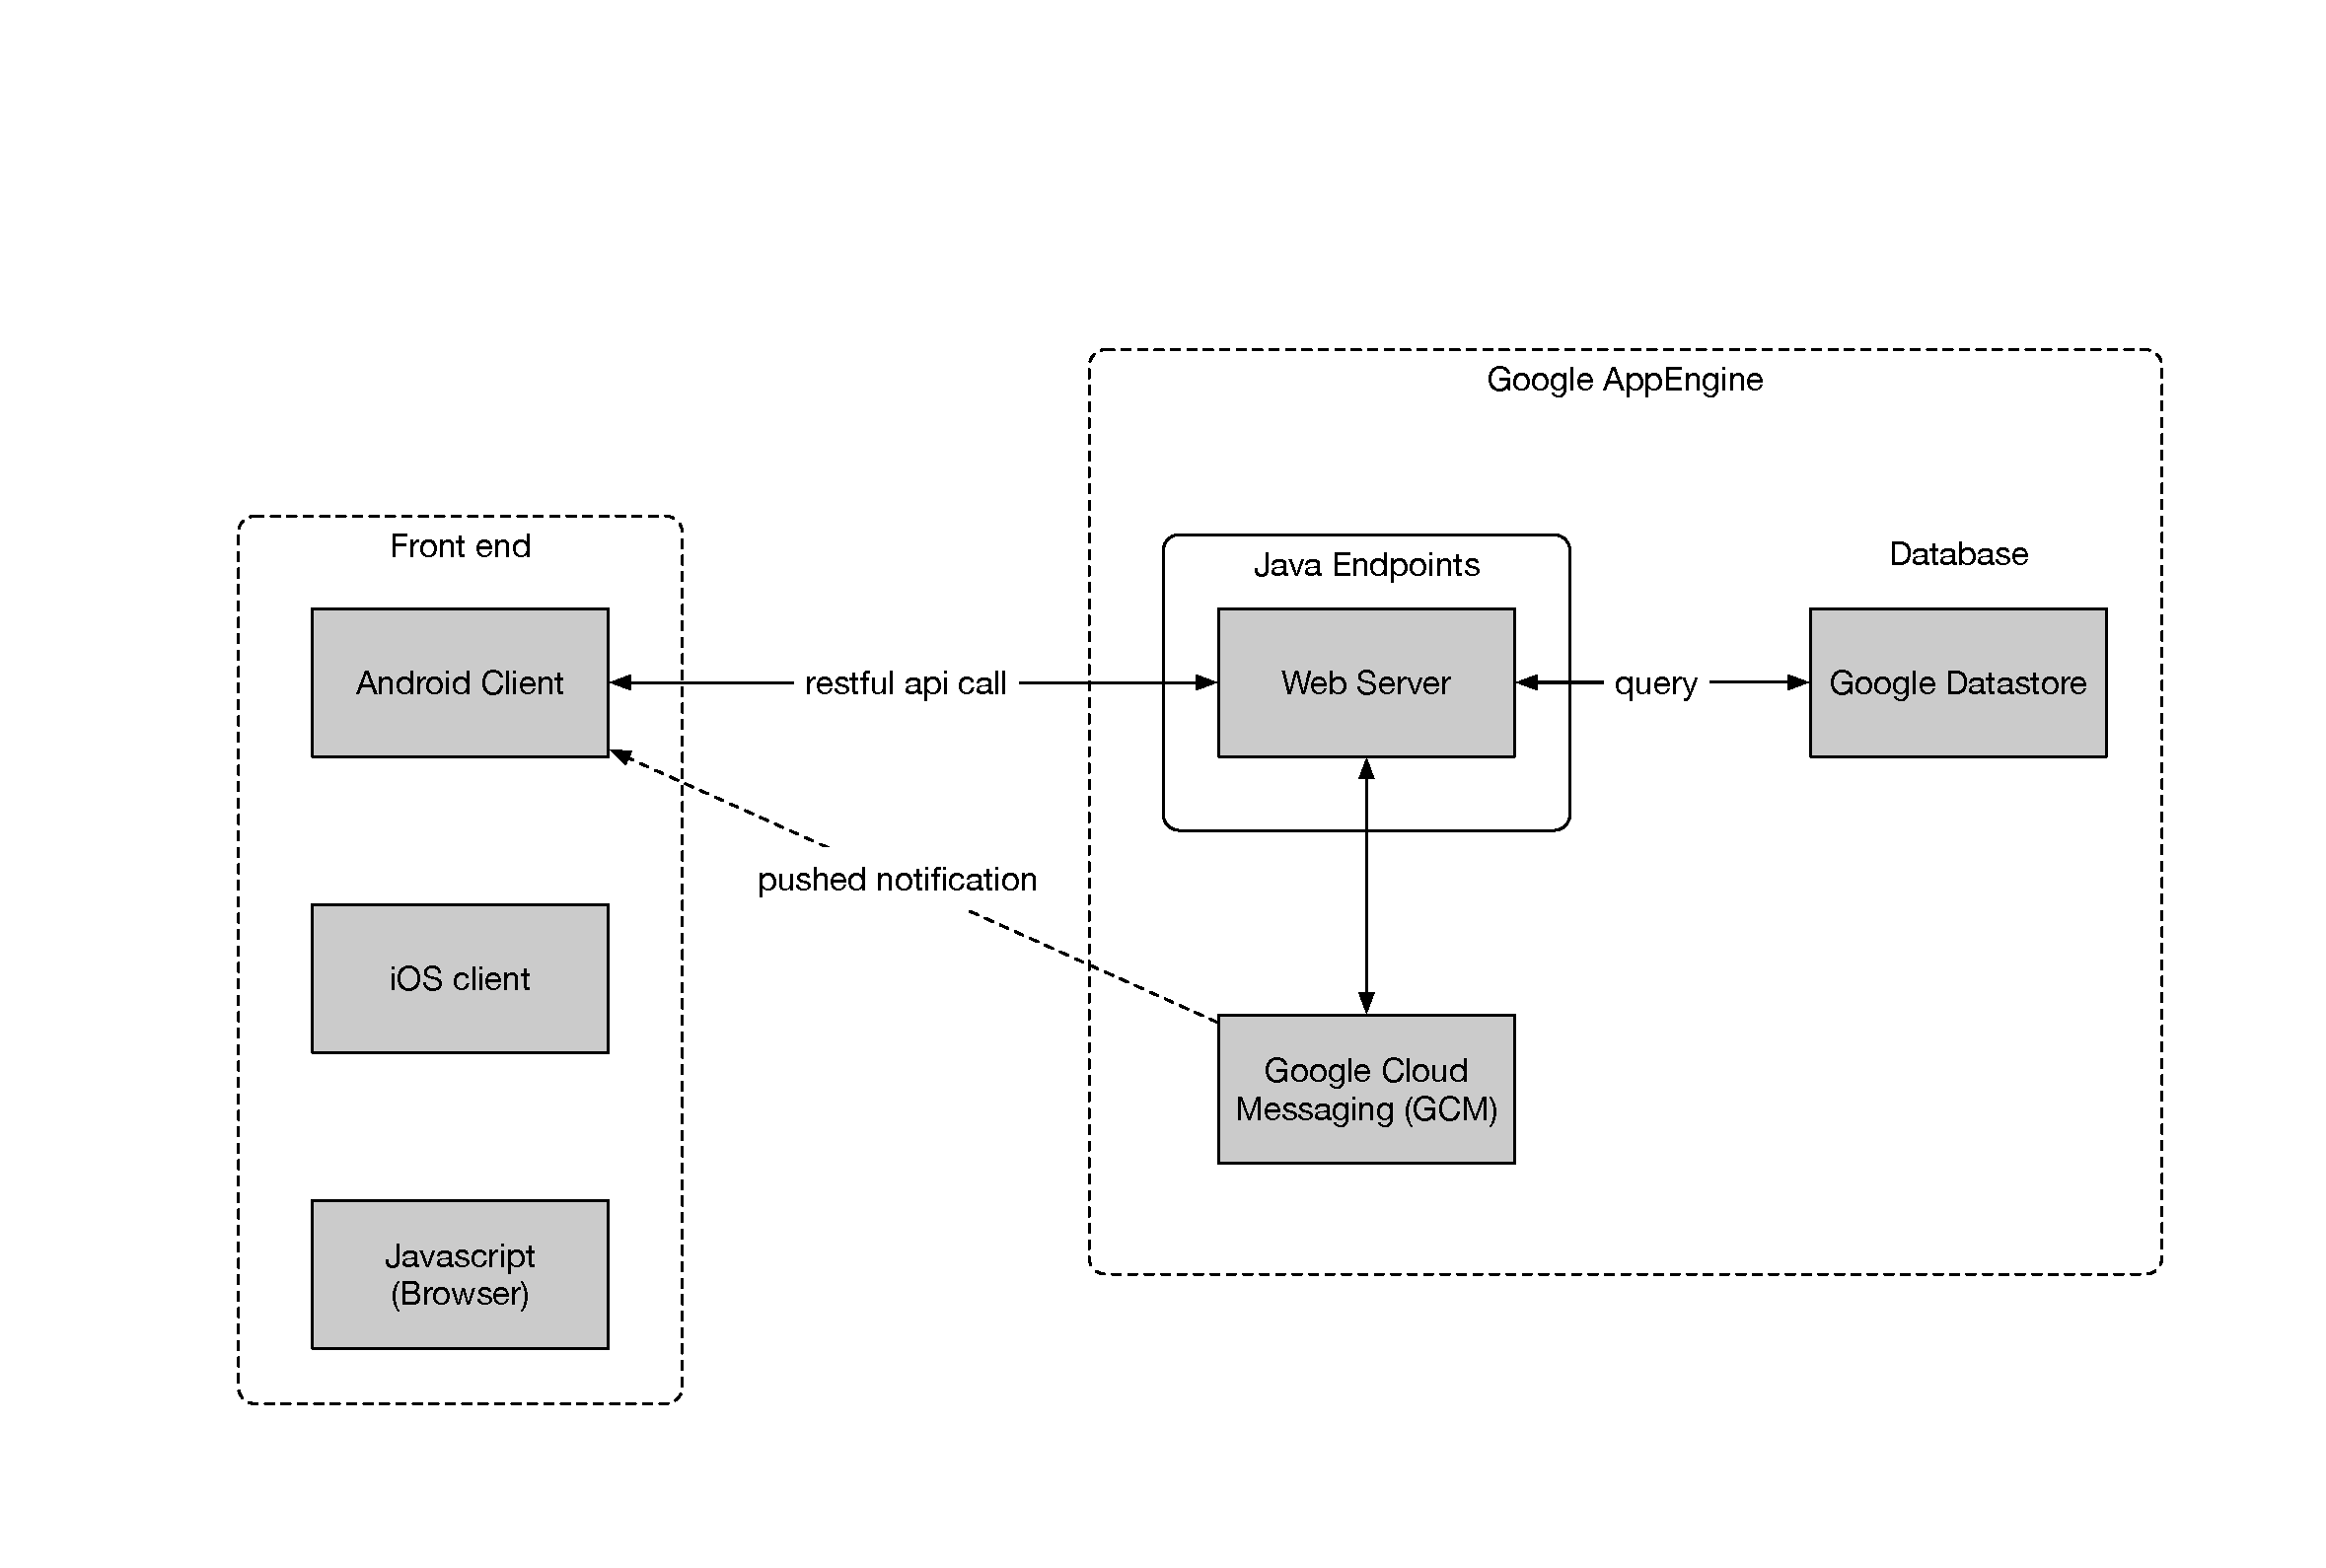
\includegraphics[width=\textwidth]{Architecture} \caption{High level architecture of the application}
\end{figure}

We hope you find write\LaTeX\ useful, and please let us know if you have any feedback using the help menu above.
\section{Work done so far} \label{sec:Work done so far} In the first half of the project, the basic application was
implemented on both server side and client side \subsection{Client side}

\begin{enumerate}
    \item Login of users using Google account.
    \item Displaying of numerical data with different choice of view including by day, by week and by month.
    \item Displaying of numerical data from different users selectively.
    \item Selectively fetching of new data from backend.
    \item Displaying of other users and subscription mechanics.
\end{enumerate}

\subsection{Server side}

\begin{enumerate}
    \item Implemented a RESTful API for different features on the application including:
    \item Subscribing and Un-subscribing
    \item Posting and Retrieving of Data
    \item Register of new users and devices
    \item Sending Notification messages to users via Google Cloud Messaging
\end{enumerate}

\subsection{Android development practices}
In order to approach the latest change in new Android version and Android SDK, the project aims to use the latest tools
and practices suggested by Google. The client side application was made with consideration about design and components
choices.

\subsection{Software engineering practices}
Different standards in software engineering was considered and followed throughout the development of the application so
that the code can be read and reused by other developers.Serious consideration and effort has been put in the designing
the graph components such that the application can be easily extended to other types of data i.e. blood pressure, blood
sugar etc. as well as different ways of viewing data in the future.

\section{Future work} \label{sec:Work done so far}
Although the core codebase has been completed, there are space for improvement for this project.
\subsection{Features}
\begin{enumerate}
    \item Notifications pushing depending on the data flow to make the application more
        user-friendly
    \item Implementing display view of different types of data
    \item (Optional) Connecting with real measuring devices
        to complete the full-stack solutionImplementation
\end{enumerate}

\subsection{Implementation}
Fixing of remaining bugs in the application

\subsection{Software engineering practices}
Refactor if necessary to have a clean and loosely coupled code base so that it can be reused and integrated with other projects

\section{Conclusion}
In conclusion, the core code base of the project has been completed but there are still features to
be implemented to provide a better interaction with the users.On the other hands, consideration in software engineering
practices and latest change of Android library is also required throughout the process of development for the rest of
the project.
\end{document}
